\chapter{Attitude Estimation}
\label{chap:kf}

\section{Introduction}
\begin{figure}[!h]
\centering
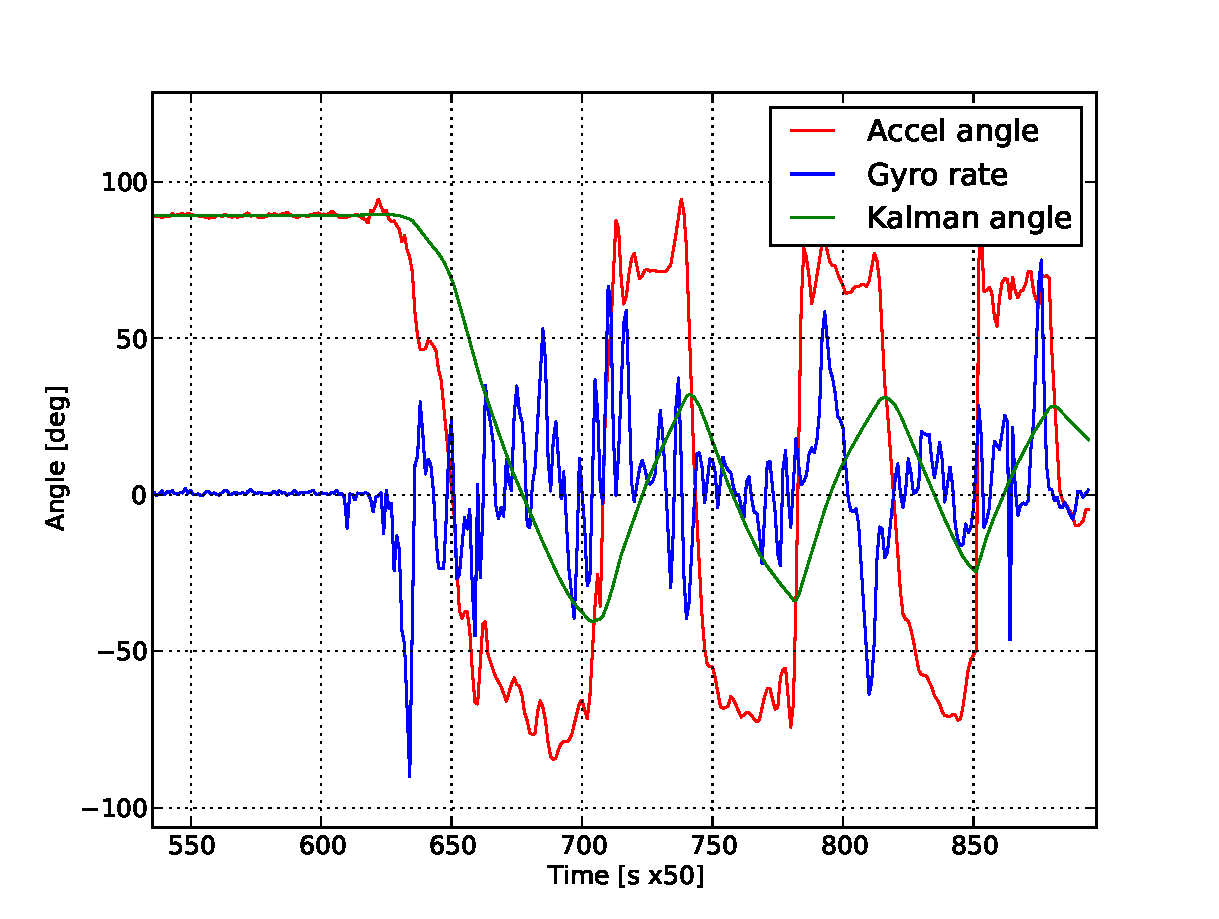
\includegraphics[scale=0.8]{fig/kalman_lowfreq.pdf}
\caption{Kalman filter : Low frequency input}
\label{fig:5_kalman_lowfreq}
\end{figure}
As shown in Fig. \ref{fig:5_kalman_lowfreq}, the readings of the gyroscope and the accelerometer
are highly noisy and erratic even in the situation of smooth movements of the IMU. This shows,
that depending upon either of the two sensors is not good for pitch estimation. Gyroscopes are
high frequency sensors and accurately estimate the rate. However, they also show pronounced
variation of readings with time (gyro bias) and temperature (compensated to an extent). 
Accelerometers are good at low frequency measurements. These do not suffer from a growing
bias like the gyroscopes and can be used to correct the readings estimated on the basis of
gyroscope rate from time to time. We look at Kalman filter as a way to fuse these two sensors.\\

Various alternatives for filtering schemes exist and complementary filters are very widely used
for fusing accelerometers and gyroscopes on IMUs. I decided to use a Kalman filter because
the micro-controller can easily handle the computations at usable update rates of about
20-50 Hz. This is one of the major reasons cited in literature for the use of complementary
filters over Kalman filters. It is also noted that for linear systems, there is little difference in the equations of the two filters.\\

\section{Equations}
The equations for Kalman filter with a state vector $\bm{x} = [x_1\;\;x_2]^T = [\theta\;\;\dot{\theta}]^T$ are give below.\\

State equation :
\begin{equation}
\label{eqn:5_kalmanstate}
\bm{x}_{k+1} = \bm{A}\:\bm{x}_k + \bm{B}\:\bm{u}_k + \bm{w}_k
\end{equation}
Output equation :
\begin{equation}
\label{eqn:5_kalmanop}
y_{k+1} = \bm{C}\:\bm{x}_{k+1} + z_{k+1}
\end{equation}
Update equations :
\begin{equation}
\label{eqn:5_kalmanK}
\bm{K}_k = \bm{A}\:\bm{P}_k\:\bm{C}^T\:\left( \bm{C}\:\bm{P}_k\:\bm{C}^T + S_z\right)^{-1}
\end{equation}
\begin{equation}
\label{eqn:5_kalmanhat}
\hat{\bm{x}}_{k+1} = \left( \bm{A}\:\hat{\bm{x}}_k + \bm{B}\:\bm{u}_k \right ) + \bm{K}_k\:\left ( y_{k+1} - \bm{C}\:\hat{\bm{x}}_k\right)
\end{equation}
\begin{equation}
\label{eqn:5_kalmanP}
\bm{P}_{k+1} = \bm{A}\:\bm{P}_k\:\bm{A}^T + \bm{S}_w - \bm{A}\:\bm{P}_k\:\bm{C}^T\:S_z^{-1}\:\bm{C}\:\bm{P}_k\:\bm{A}^T
\end{equation}

For our state vector, the equations consist of,
\begin{equation}
\bm{A} = \left[ \begin{array}{cc} 1& dt\\0&1\end{array}\right]\:\:\:\bm{B} = \left[ \begin{array}{c} dt\\0\end{array}\right]\:\:\:
\bm{u} = \left[ \begin{array}{c} \dot{\theta}_{gyro}\\0\end{array}\right]\:\:\:y = \theta_{accel}\:\:\: \bm{C} = \left[ \begin{array}{c} 1\\0\end{array}\right]
\end{equation}
$\bm{P}$ is called the estimation error co-variance and can be initialized to some value, a small value implies that we expect the
error co-variance to be small too. We assume that the estimation errors are completely dependent upon one another and hence
initialize the matrix as identity. $S_z$ is the accelerometer variance obtained from the datasheet. $\bm{S}_w$ is the gyroscope
covariance matrix. Let $\nu_{angle} = dt\:\sigma_{rate}$ and $\nu_{rate} = 0$. These values are thus obtained from the datasheet
for a particular filter update rate.
\begin{equation}
\bm{P} = \left[ \begin{array}{cc} 1& 0\\0&1\end{array}\right]\:\:\:\bm{S}_w = \left[ \begin{array}{cc} \nu_{angle}^2 &\nu_{angle}\:\nu_{rate}\\ \nu_{angle}\:\nu_{rate}&\nu_{rate}^2\end{array}\right] = \left[ \begin{array}{cc} 
92\times10^{-6} &0\\0&0\end{array}\right]
\end{equation}
Eqns. \ref{eqn:5_kalmanstate} -- \ref{eqn:5_kalmanhat} were converted to their algebraic 
form instead of the matrix operations for better calculation speed. Fig. \ref{fig:5_kalman_lowfreq} shows the performance of this
filter with calculations being done on the computer. Fixed-point arithmetic has been implemented on the micro-controller and will
be used for the onboard Kalman filter.

\section{Results}
\begin{figure}[!h]
\centering
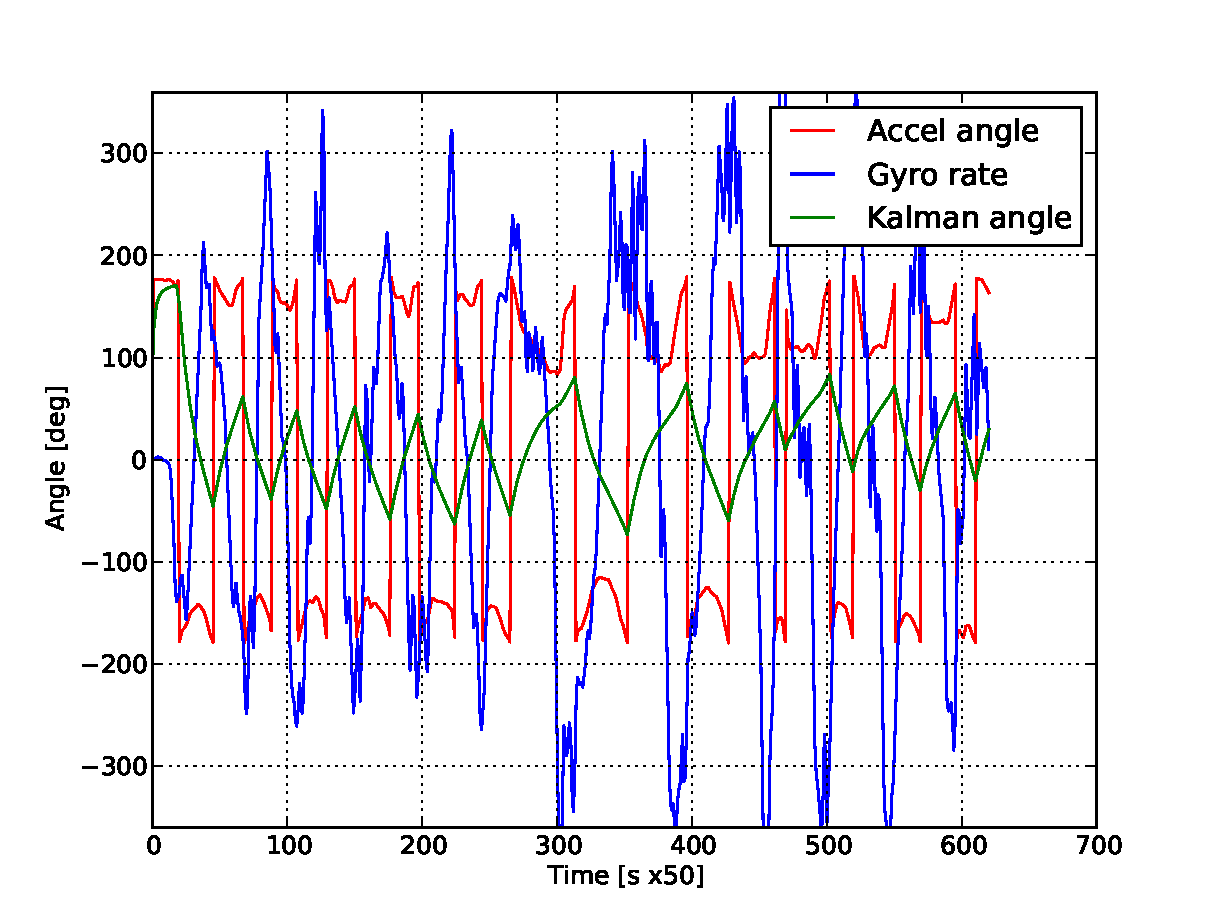
\includegraphics[scale=0.8]{fig/kalman_highfreq.pdf}
\caption{Kalman filter : High frequency input}
\label{fig:5_kalman_highfreq}
\end{figure}
Fig. \ref{fig:5_kalman_highfreq} has been plotted for a very high frequency movement of the IMU. As shown, the rates exceed 
$\pm320^o/s$ which is the maximum rate detected by the gyro. The final output of the kalman filter does match the hand movement
of about 90 degrees. However, at about the $300^{th}$ update, it completely misses a very fast 360 deg. rotation of the IMU. This
is reasonable because even the accelerometer and gyroscope do not seem to significantly register this movement.

\begin{figure}[!h]
\centering
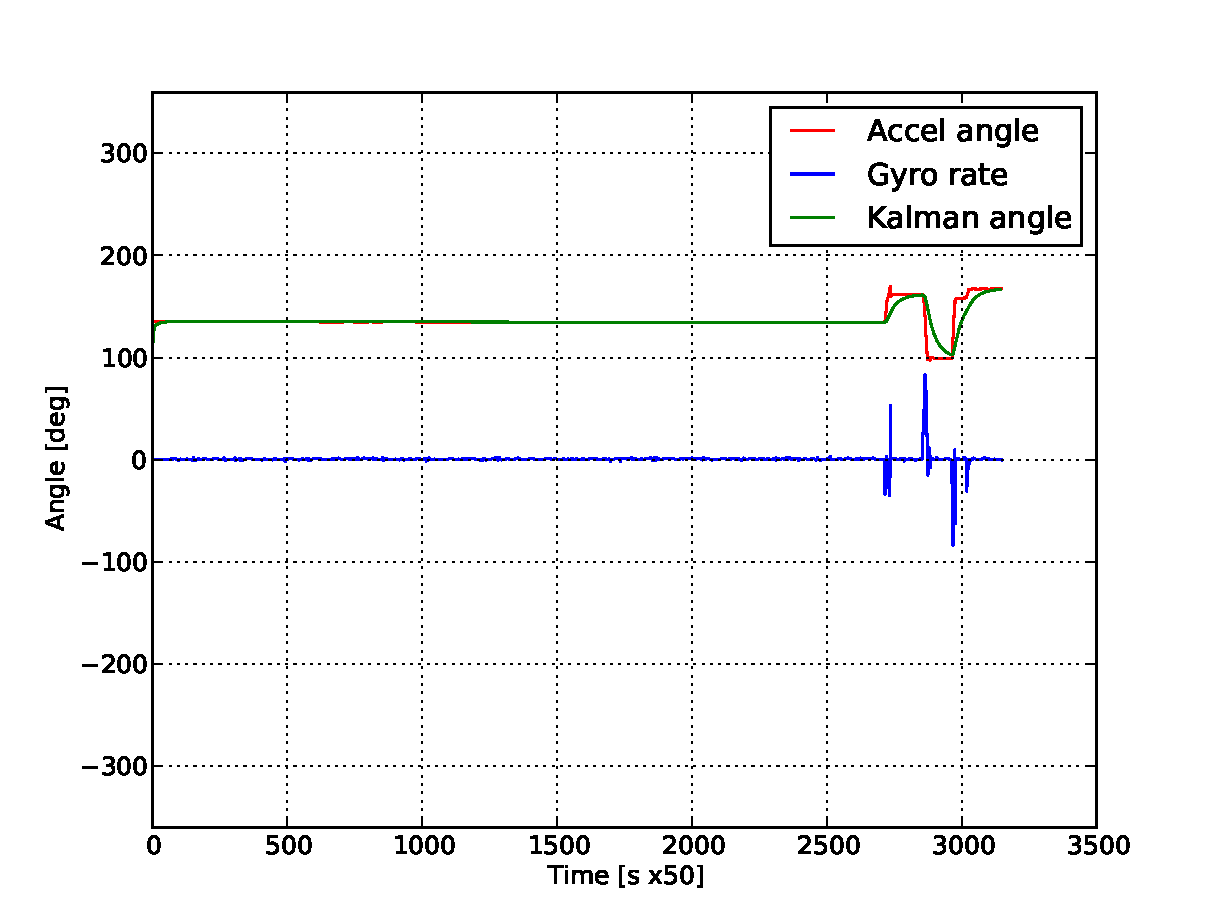
\includegraphics[scale=0.8]{fig/kalman_drift.pdf}
\caption{Kalman filter : Gyro drift}
\label{fig:5_kalman_gyrodrift}
\end{figure}
\newpage
Fig. \ref{fig:5_kalman_gyrodrift} shows readings plotted for 5 minutes at a 10 Hz update rate for the filter. It is seen that the
gyro rate has some noise. However, integrating this noise does not show a large error in the angle moved by the sensor. The
integral of the gyro rate is zero for all the time. The drift mentioned for gyroscopes is not to be seen even for periods as large as
12 minutes.

\section{Implementation}
We have to perform filtering on the onboard embedded system. It is essential that we finish off
the filtering part quickly so that the microcontroller can devote enough time to implementing
the control law. Polling data from the sensors also takes precious time. I set an update rate of 50 Hz
as the goal, this is also the maximum update rate of the gyroscope, so the filter cannot be run faster
than that. Two major parts of the implementation are as follows,

\subsection*{Inverse tan function}
The tilt of the accelerometer is obtained as follows,
\begin{equation}
\theta = tan^{-1} (\frac{a_y}{a_x})
\end{equation}
The C30 library provides an implementation of the $tan^{-1}$ function in floating point. However, these
operations take time on a 16-bit microcontroller. I thus implemented it using a table of stored values
and interpolating for values between them. The salient features of this are,
\begin{enumerate}
\item
\textit{tan} is an odd function, so we just need to include positive values in the table
\item
It is highly non-linear after 70 deg. So we will have a $tan^{-1}$ function only from -70 to +70 deg.
This gives a range of 140 deg. for the attitude which will be sufficient.
\item
Tangent function is linear enough till $15^{o}$, so we use this in our calculations. Divide the
interval $[$tan($15^{o}$), tan($70^{o}$)$]$ in 16 intervals. Store these \textit{tangents} and
the corresponding \textit{angles} in a table.
\item
Given a value, find out the interval within which it lies. Linearly interpolate \textit{tangent}
function within this interval.
\item
We identify a systematic``ish'' error of 0.06 deg in our implementation and hence add 0.06 deg.
while calculating the angle in the tabular implementation.
\item
This implementation requires just 48 bytes of memory and is computationally cheap as well.
\end{enumerate}
Fig. \ref{fig:5_atanD} shows the error between the $tan^{-1}$ function of the python math library
and $tan^{-1}$ function using the table above. We can implement this on the microcontroller using
fixed point arithmetic as shown in Sec. \ref{subsec:fp} to further reduce the computational time.
\begin{figure}[!h]
\centering
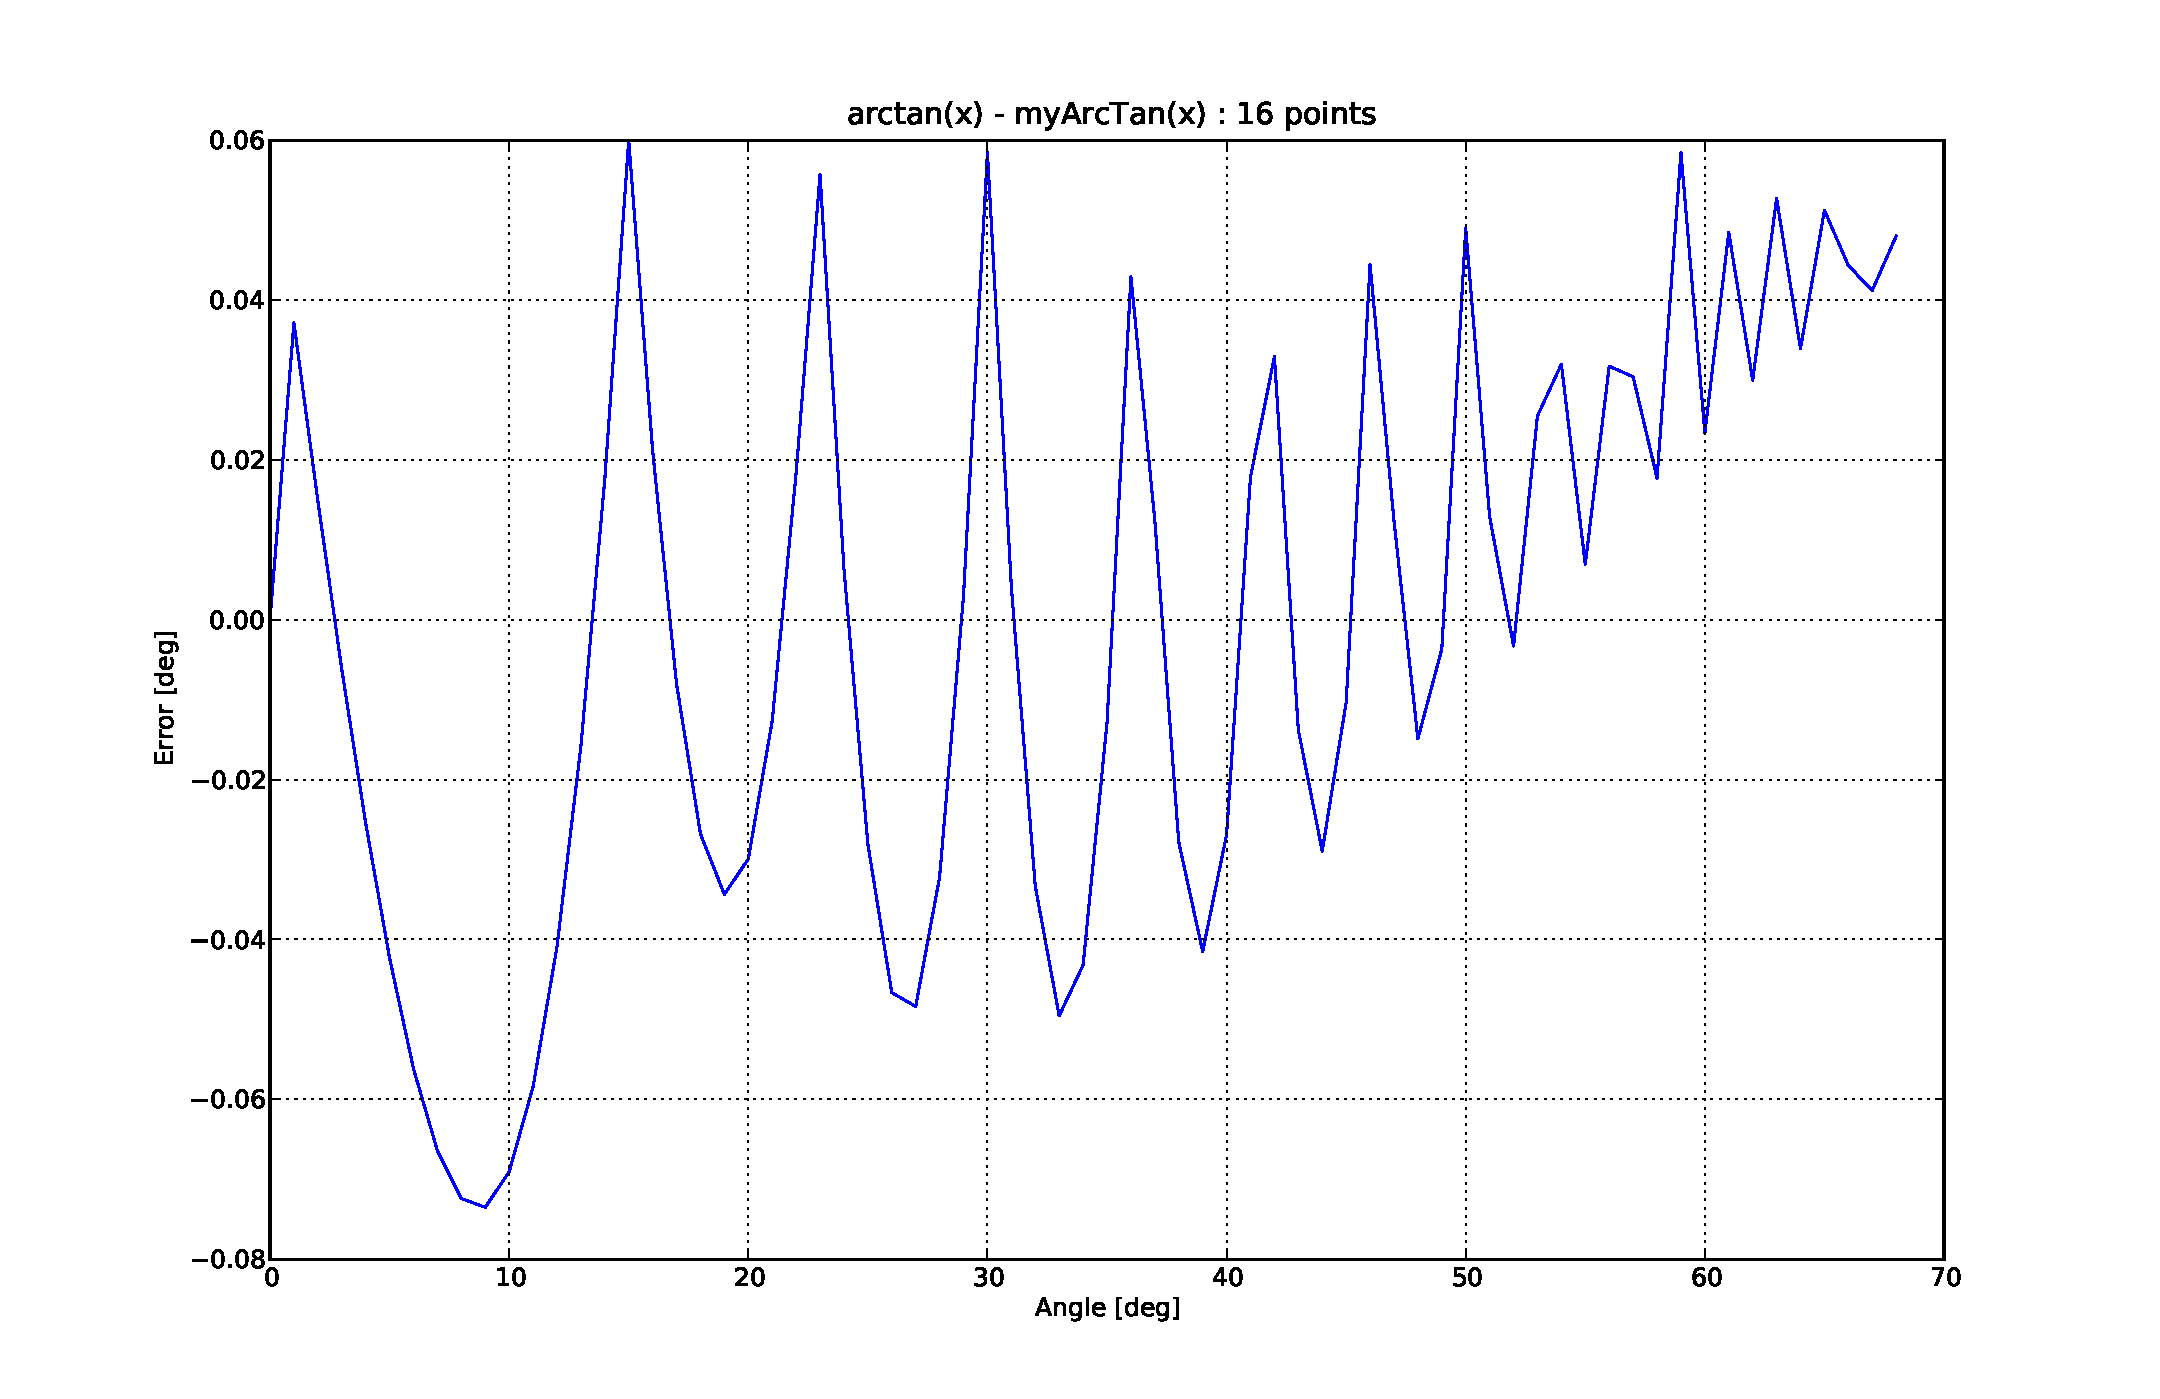
\includegraphics[scale=0.45]{fig/atanD.pdf}
\caption{$tan^{-1}$ function : Error between actual and the tabular implementation}
\label{fig:5_atanD}
\end{figure}

\subsection*{Fixed point arithmetic}
\label{subsec:fp}
There is one another way to reduce the computational overhead of the Kalman Filter. The accelerometer
provides the inclination values directly. It is known that the error in these values is $\pm0.5$ deg.
Implementing the tabular tangent function and the Kalman Filter in fixed point both is an option.
I however feel that the errors in the fixed point arithmetic will dominate over the inclinometer error
and hence it is not a bad idea to use the inclinometer directly. This will save some CPU cycles too.
Hence I implemented the Kalman Filter in fixed point arithmetic. The salient features are as follows,
\begin{enumerate}
\item
On a 16-bit microcontroller, we use 10.6 type signed fixed point numbers. The higher 10 bits are used
for the integer part of the number whereas the lower 6 bits are used for the mantissa. The
resolution of this scheme is thus $\frac{1}{2^{6}} = 0.015625$.
\item
Thus we have to scale every number by $2^{6} = 64$ before operating upon it. The Kalman
Filter constants are already hardcoded in the 10.6 form. The variables also operate and
get operated in this form itself.
\item
Multiply by 64 everytime two 10.6 fixed point numbers divide and divide by 64 everytime they get
multiplied to preserve the scaling.
\item
The integer part should be large enough to accomodate the rollover from the mantissa part after the
multiplication.
\item
Type-casting should be done properly while performing the arithmetic to prevent truncation by the
compiler.
\end{enumerate}

Figures \ref{fig:5_KF_fp_hf} and \ref{fig:5_KF_fp_lf} plot the tilt given by the accelerometers directly 
vs the fixed point implementation on the microcontroller vs the floating point implementation on a
computer. The floating point implementation on the computer
lags behind the microcontroller implementation slightly. This is probably because the covariance of the
accelerometer is a floating point number with a mantissa greater than 0.5 and is thus badly
rounded off in the fixed point implementation.
\newline
\begin{figure}[!h]
\centering
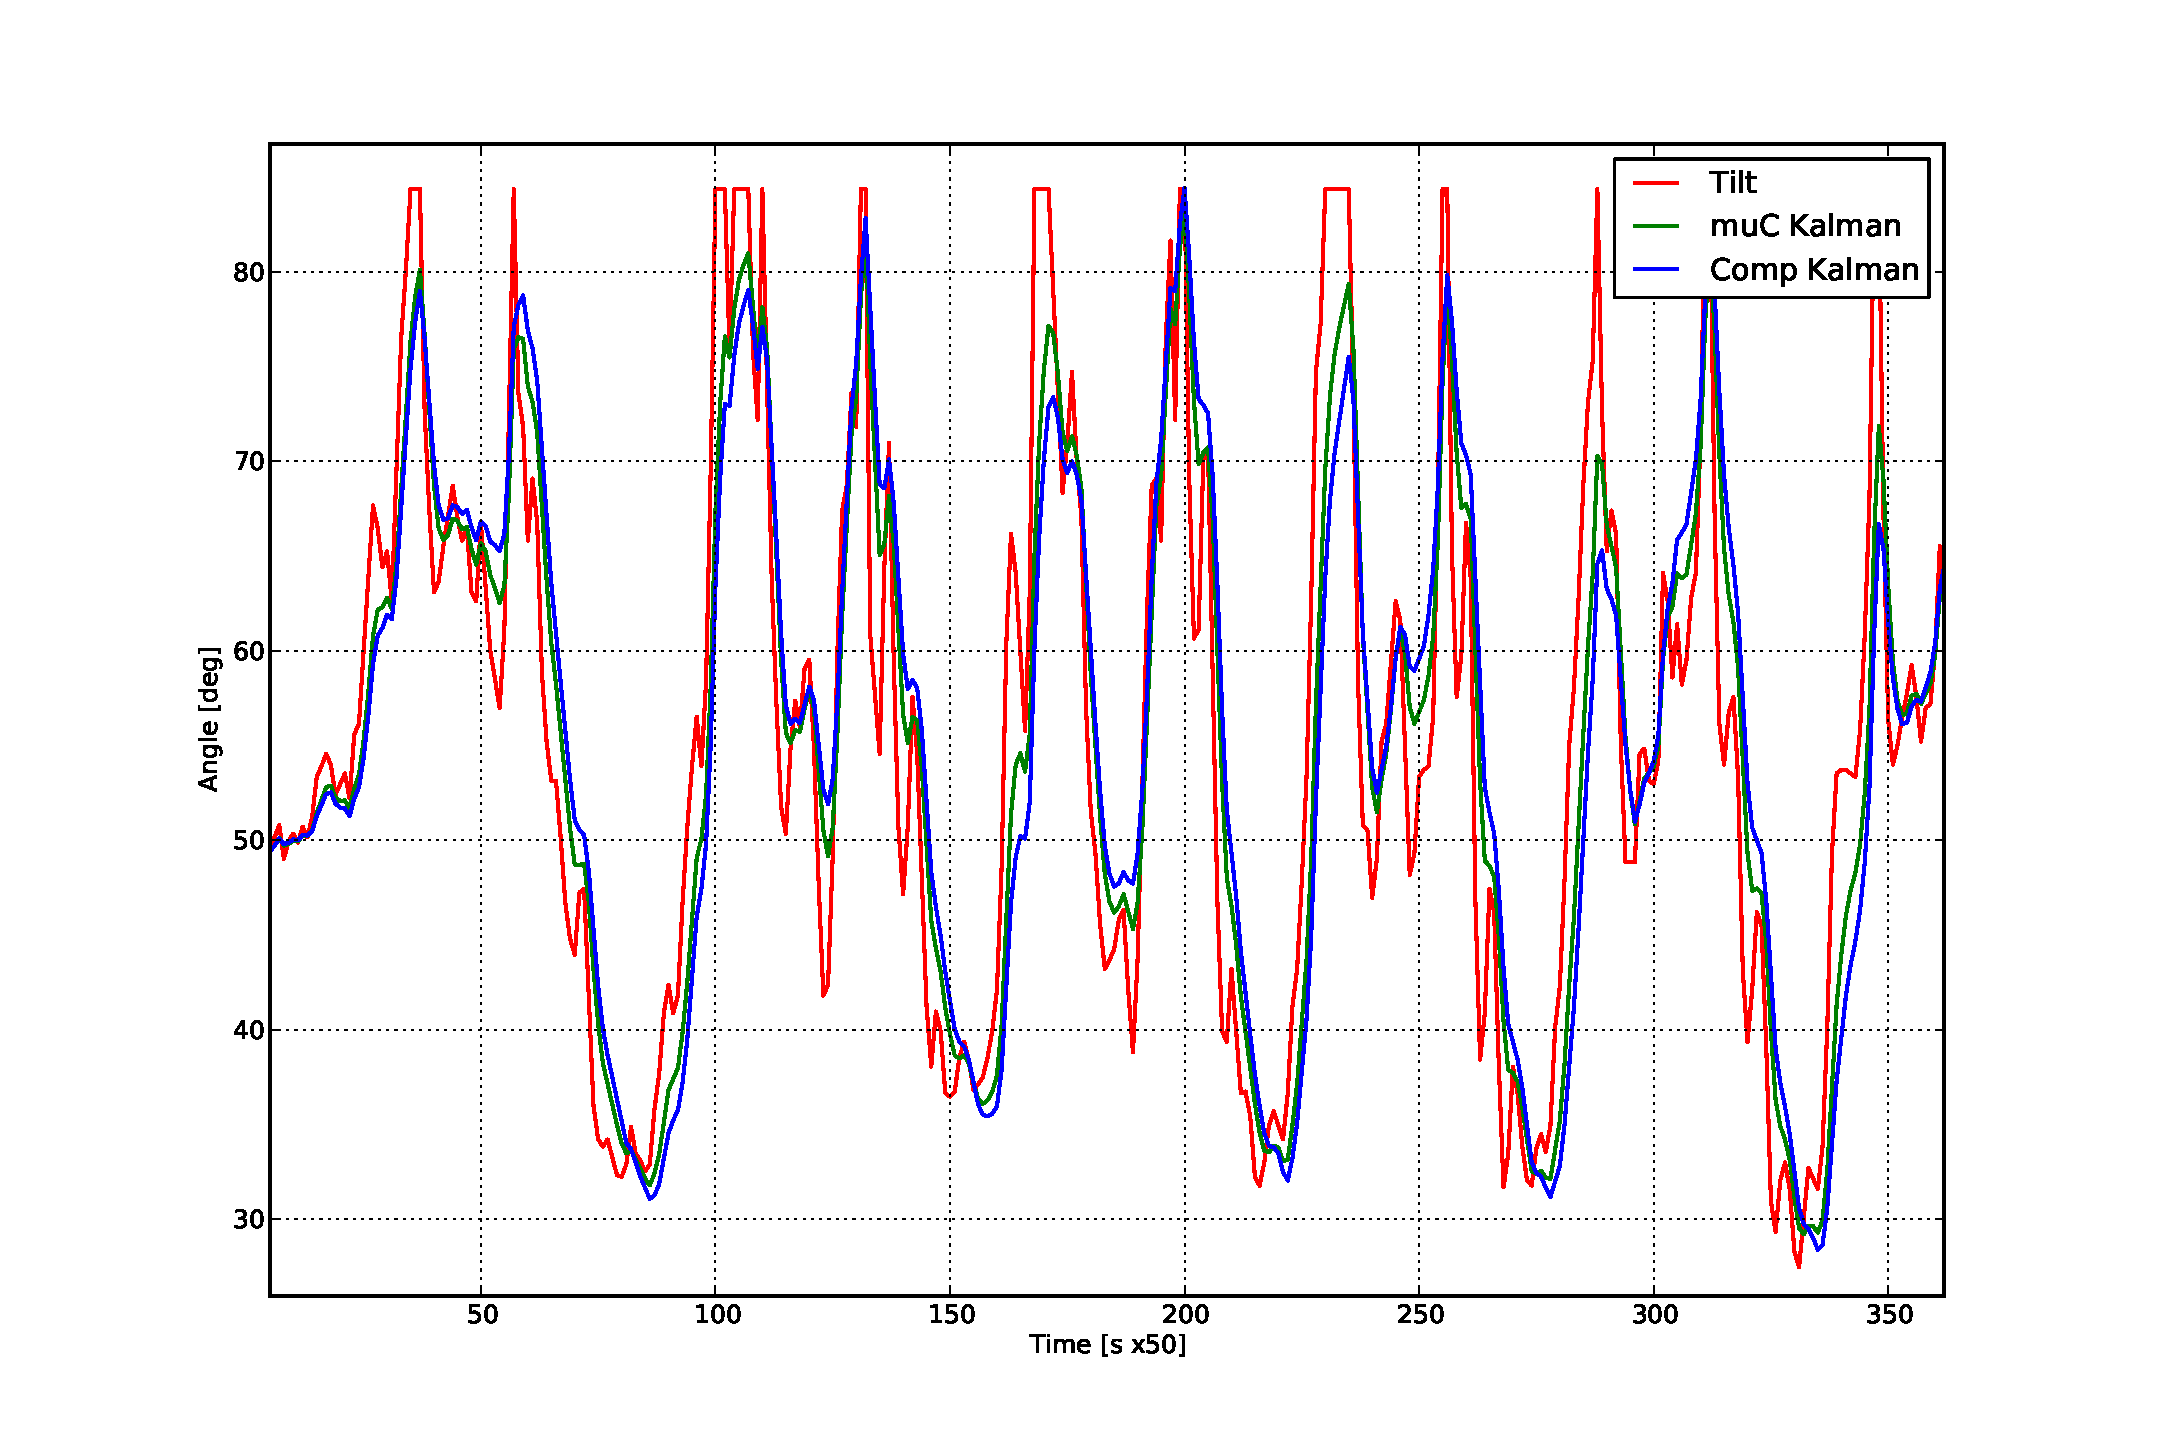
\includegraphics[scale=0.70, angle=270]{fig/kf_fp_hf.pdf}
\caption{Fixed point Kalman Filter : High freqency}
\label{fig:5_KF_fp_hf}
\end{figure}
\begin{figure}[!h]
\centering
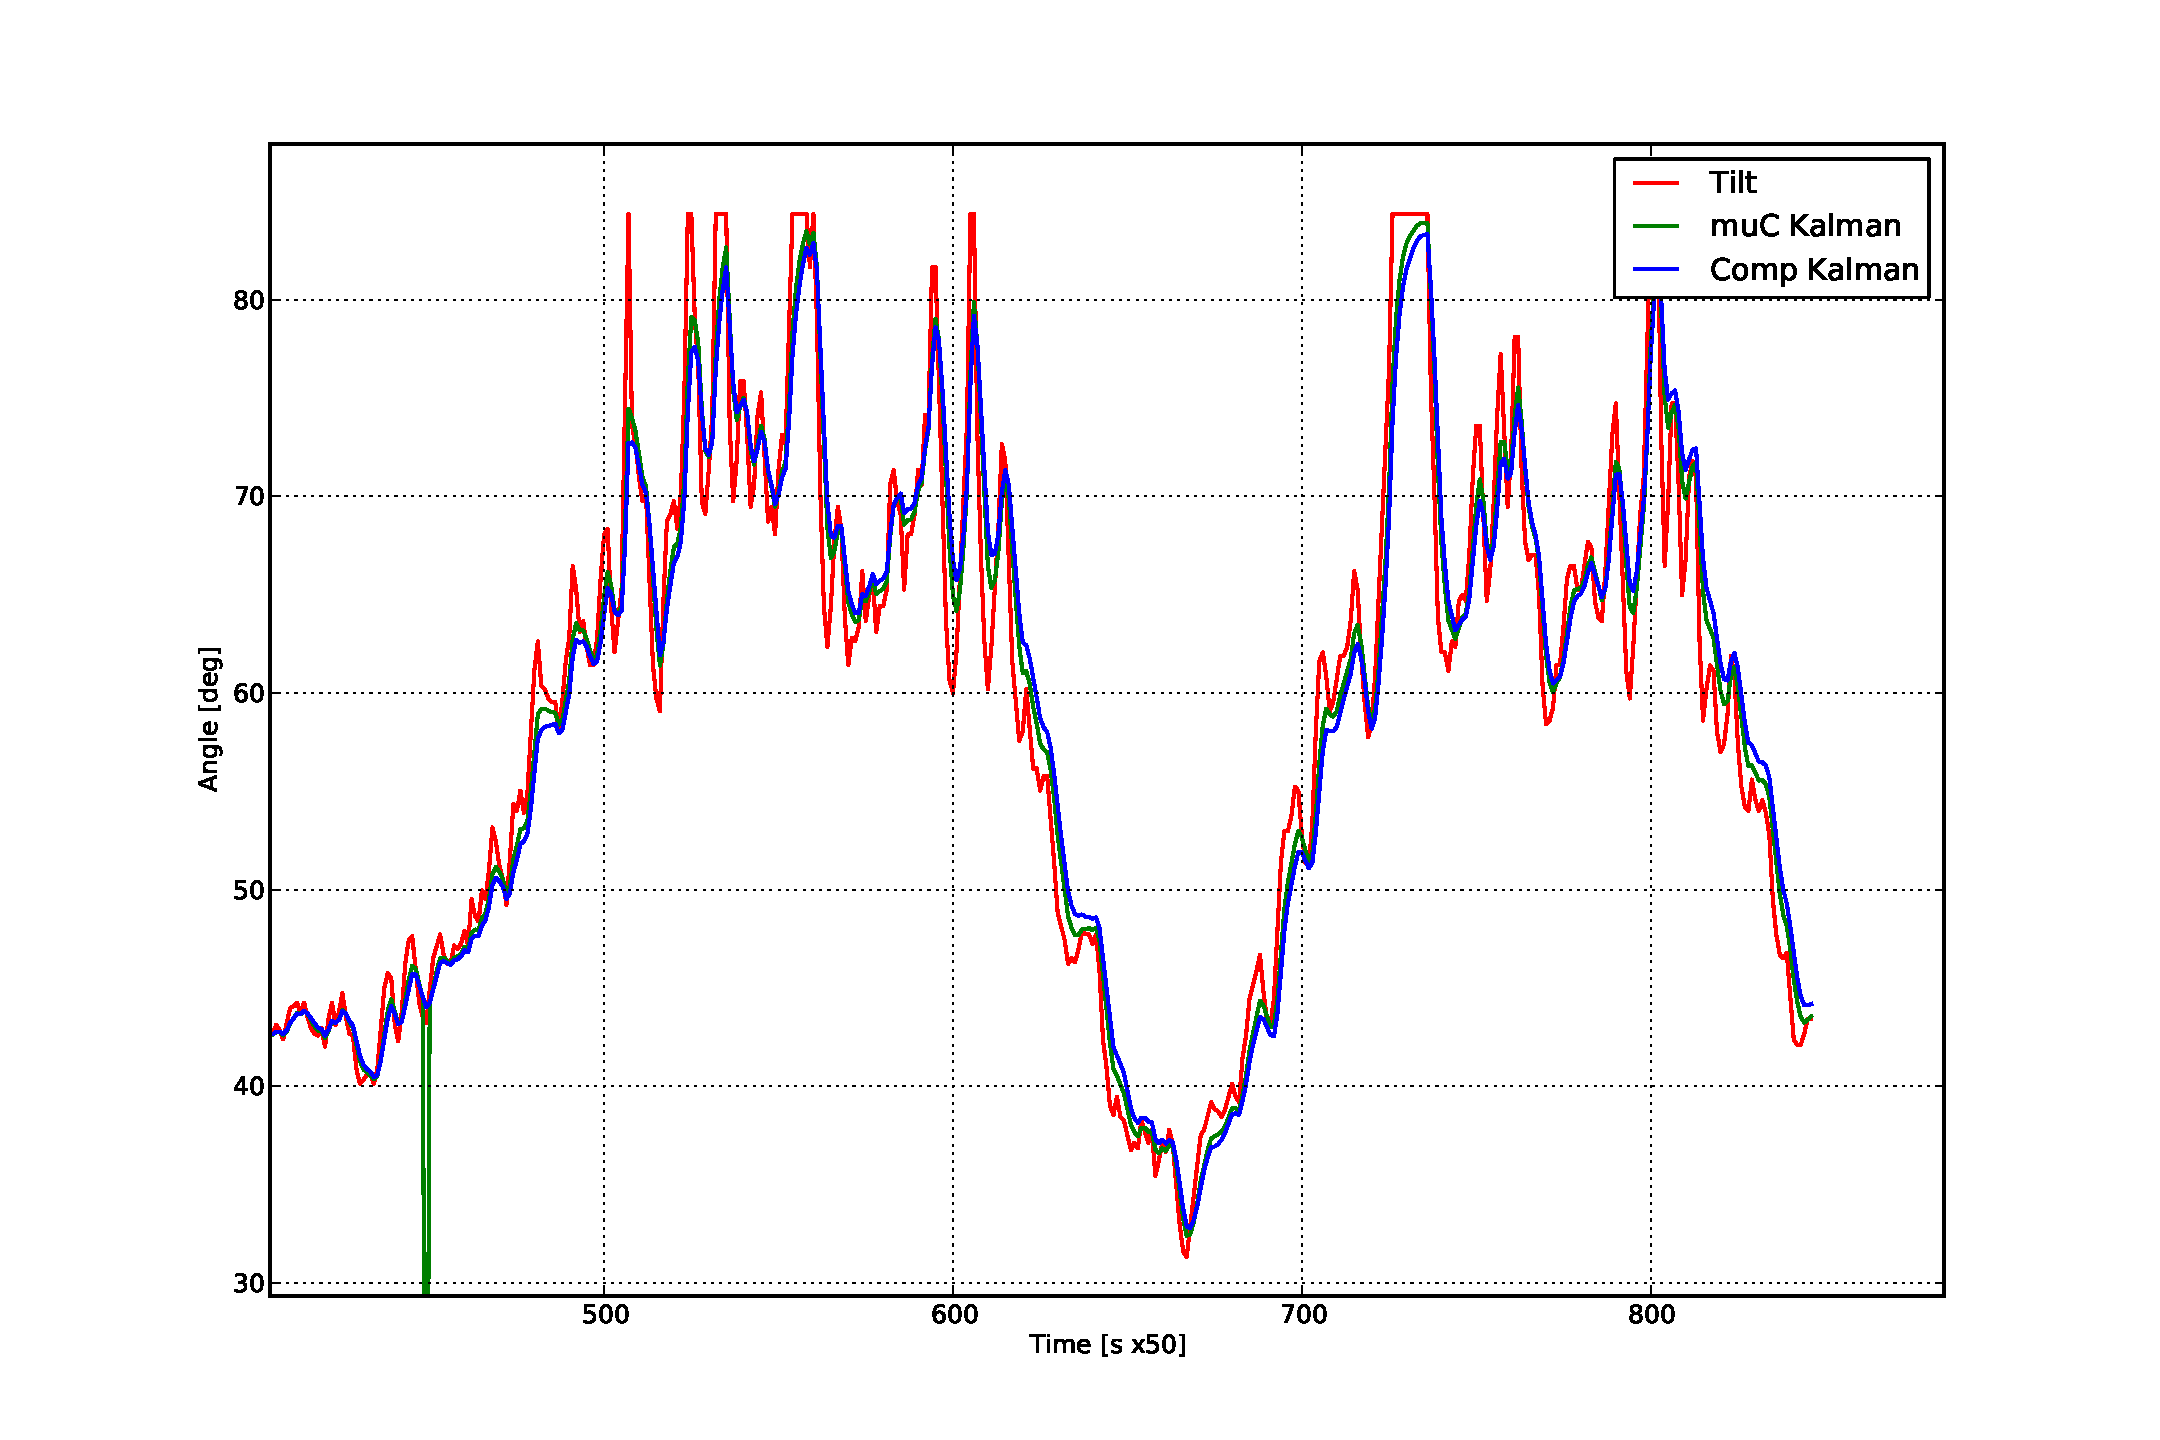
\includegraphics[scale=0.70, angle=270]{fig/kf_fp_lf.pdf}
\caption{Fixed point Kalman Filter : Low freqency}
\label{fig:5_KF_fp_lf}
\end{figure}

The source code for the fixed point implementation is given in the appendix.
















